\capitulo{5}{Aspectos relevantes del desarrollo del proyecto}

Lo más relevante de este proyecto es el transformar la última versión de Thoth a una aplicación web hecha por medio de GWT lo que supone comprender el funcionamiento interno del Thoth original, <<desglosándolo>> para poder adaptarlo a las condiciones de un proyecto hecho con GWT.
Estas condiciones limitan un poco la aplicación y nos obligan a reformar partes que antes eran más sencillas.

Además de condicionar Thoth a GWT, también hemos añadido nuevas funcionalidades de las que hablaremos y que completan la aplicación.



\section{Internacionalización}
La aplicación cuenta con la funcionalidad de la internacionalización. Dentro del menú se pueden elegir entre varios idiomas a los que se traducirán los diferentes elementos. Los idiomas en los que está disponible la versión web de Thoth son: alemán, castellano o español, francés y por supuesto inglés. Consideramos que esta funcionalidad es muy importante para poder llegar a diferentes países en el caso de que fuera necesario.

La internacionalización de la aplicación es un poco diferente a la utilizada en la versión de escritorio de Thoth. En primer lugar es necesario incluir una interfaz con los métodos para la internacionalización y los mensajes <<por defecto>> asociados a cada uno. Cada vez que queramos hacer uso de esos mensajes hay que hacer una llamada al método de la interfaz. Esa interfaz se encuentra en el directorio <<client.gui.utils>> donde se encuentran también los ficheros <<properties>> asociados, donde se encuentran las diferentes traducciones según el mensaje. Estos mensajes son los mismos que los utilizados para la internacionalización de Thoth V2.

Para poder realizar el cambio de idioma es necesario hacer uso de las propiedades las clases <<xml>> y <<html>> de GWT, en concreto <<locale>> que es la que especificará la localidad, que determina el idioma. Por ello cada vez que elegimos un idioma, la aplicación se redirige a una nueva <<URL>> (llevando a cabo una nueva compilación) con el atributo \texttt{locale=} seguido de las siglas del idioma al que se quiere traducir.

\section{Google Web Toolkit}

Para trabajar con GWT hemos utilizado el entorno de desarrollo de eclipse y con ayuda del \emph{plugin} de Google, se crea un proyecto. Al crear un proyecto con él, se crean unos paquetes por defecto:
\begin{itemize}
\item Client: las clases dentro de este paquete se traducirán a lenguaje JavaScript. Es la parte fundamental de un proyecto en GWT y en ella se encuentra la clase principal que implementa <<EntryPoint>>  (indicativo de que es la clase en la que se encuentra la función principal) y la función principal <<onModuleLoad>>. Todo proyecto tiene al menos una clase en el cliente con estas características.
\item Server: dentro, las clases no se traducirán a JavaScript y se puede programar en Java de forma completamente normal. Para realizar la comunicación se utilizan llamadas de procedimiento remoto (Remote Procedure Calls). Incluye servelets, bases de datos etc.
\item Shared: mezcla de las dos anteriores. Se traduce también a JavaScript y puede ser utilizada en ambos lados de la aplicación. Suelen ser clases de ayuda para las acciones de un lado al otro de la aplicación.
\end{itemize}

\subsection{Módulos en GWT}

Las unidades individuales de configuración en GWT se denominan módulos. Un módulo agrupa todos los parámetros de configuración que necesita su proyecto GWT:

\begin{itemize}

\item Módulos heredados.
\item Un nombre de clase como punto de entrada. Estos son opcionales, aunque cualquier módulo referido en HTML debe tener al menos una clase de punto de entrada especificada.
\item Entradas de ruta de origen
\item Entradas de ruta pública
\item Reglas de vinculación diferida, incluyendo proveedores de propiedad y generadores de clase

\end{itemize}
Los módulos están definidos en archivos con extensión <<.gwt.xml>>. En una aplicación con varios módulos como la nuestra, hay dos formas de enfocarlo: compilando cada módulo por separado o creando una definición XML de módulo de nivel superior que incluya todos los módulos y compilar el módulo de nivel superior.

\subsection{Comunicación RPC}

Como ya hemos hablado, RPC se utiliza para transferir objetos Java entre el cliente y el servidor a través de HTTP. Cada vez que se transfieran objetos a través de RPC, deben ser serializados. Los pasos para establecer la comunicación consisten en crear lo siguiente:


Hay que tener en cuenta que por defecto se crea un archivo dentro del directorio <<War>> denominado <<web.xml>>. En él se configura el lugar donde se alojan los servlets, que contienen la implementación del servicio.


\subsection{Aspectos del diseño con GWT}

El diseño en GWT es uno de los apartados donde más se ha notado lo anticuado que está. Los elementos o widgets tienen diseños algo desactulizados. En realidad, esto no es un problema, ya que por medio de estilos <<css>> podemos configurar el diseño que queramos, pero es una clara desventaja en comparación con otros frameworks.

En nuestro caso, hemos hecho uso de un tema que proporciona GWT. Sirve para que al incorporarlo a un módulo con la sentencia <<\textit{inherits}>>, da un mínimo de aspecto a los elementos que se incorporen. Es el caso del módulo <<GramaticaCS>> que incorpora un tema denominado <<Clean>>. Como se pude apreciar en la siguiente imagen \ref{fig:5.1}, el estilo Clean otorga unos valores al elemento del menú, pero yo los cambio por medio de mi estilo <<GrmaticaCS.css>>. Digamos que los sobrescribo. En este caso no utilizo por tanto Clean pero para otros elementos sí.

\begin{figure}[h]
\centering
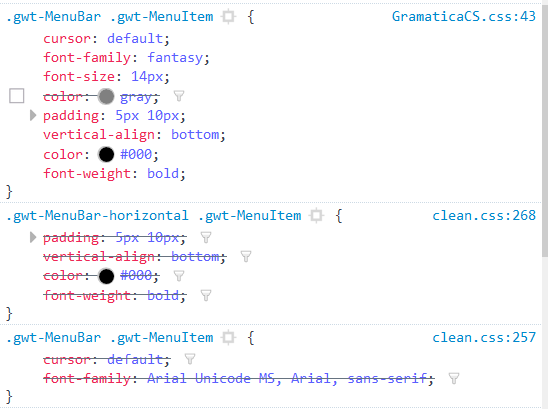
\includegraphics[width=0.70\textwidth]{estilos-css}
\caption{Vista de los estilos aplicados sobre un botón del menú desde el navegador.}
\label{fig:5.1}
\end{figure}

Es importante a la hora de diseñar, ya que la jerarquía, se aplica de más concreto a más amplio. Así si un botón está, por ejemplo, en un panel vertical y el panel vertical tiene un formato de texto stilo1 y el botón tiene otro denominado stilo2, se aplicará el stilo2. En el caso de haber un tema heredado por un módulo, hay que tener en cuenta esto para ver porqué no se ha aplicado el stilo1 a mi botón cuando yo le he dado uno al panel que lo engloba. Por defecto, al crear una aplicación con GWT, nuestro módulo hereda el estilo Standard. 

Mencionar también que algunos elementos tienen fallos que no están resueltos y como hemos visto en foros, llevan tiempo sin resolver como es el caso del TabPanel o el TabLayoutPanel. Al tratar de crear <<pestañas>> e insertar en ellas un panel con ayuda de la función insert, la vista fallaba y al añadir una pestaña nueva, borraba la anterior. Estuvimos intentándolo durante dos \emph{sprints} pero hasta que vimos que no se podía hacer de esa forma.

\section{Registro e inicio de sesión de usuarios}

En un primer momento, la aplicación se ejecutó en modo local desde Eclipse, de forma que para ello, como se explica en los anexos, necesitábamos hacer uso de la ejecución en modo \emph{Super Dev}. La base de datos era local y se podía acceder a ella añadiendo a la url local <<\_ah/admin>>.

Más tarde, una vez se conseguido hacer todo en modo local, la aplicación se despliega en  App Engine, así como todo lo que concierne a esta, es decir, base de datos, comunicación RPC, inicio de sesión etc. Todo esto se explica con más detalle en el Anexo del manual de programador.

Sin duda la parte más importante en el registro e inicio de sesión está en el servidor. Al hacer el registro tuvimos que aprender de forma detallada la relación que hay entre los módulos y el servidor. Para ello hay que meditar sobre cómo debe ser la arquitectura de acuerdo a nuestro objetivo. En esta aplicación, tenemos un módulo sólo para el registro e inicio de sesión, que se conecta a un servicio en el \emph{server}. Este servicio debe apoyarse en otro, que controlará la sesión para acceder al otro módulo que es el que contiene la gramática.

Realizar esto es una tarea ardua ya que para probar los cambio debíamos recompilar el proyecto cada vez, ejecutarlo en el navegador y comprobar los cambios añadiendo salidas por pantalla o mensajes de error. 

Con todo esto he podido aprender la forma de trabajar desde un lado, digamos, más común como sería el cliente, y comunicarlo con el servidor, que necesita ayudarse de interfaces y clases dedicadas únicamente a la comunicación entre ambos. 

El despliegue también ha sido una parte importante, que personalmente me llevó tiempo, pero que al final logramos encontrar y estamos bastante contentos con ello. 
